\section{Chosen Application Architecture}

\section{Proposed Architecture}

After investigating the alternatives, the following architecture was selected to build the tool upon. Due to the size of the graph, requirements were split to functional- (figure \ref{fr}) and non-functional (figure \ref{nfr}) requirements  

\begin{figure}[p]
	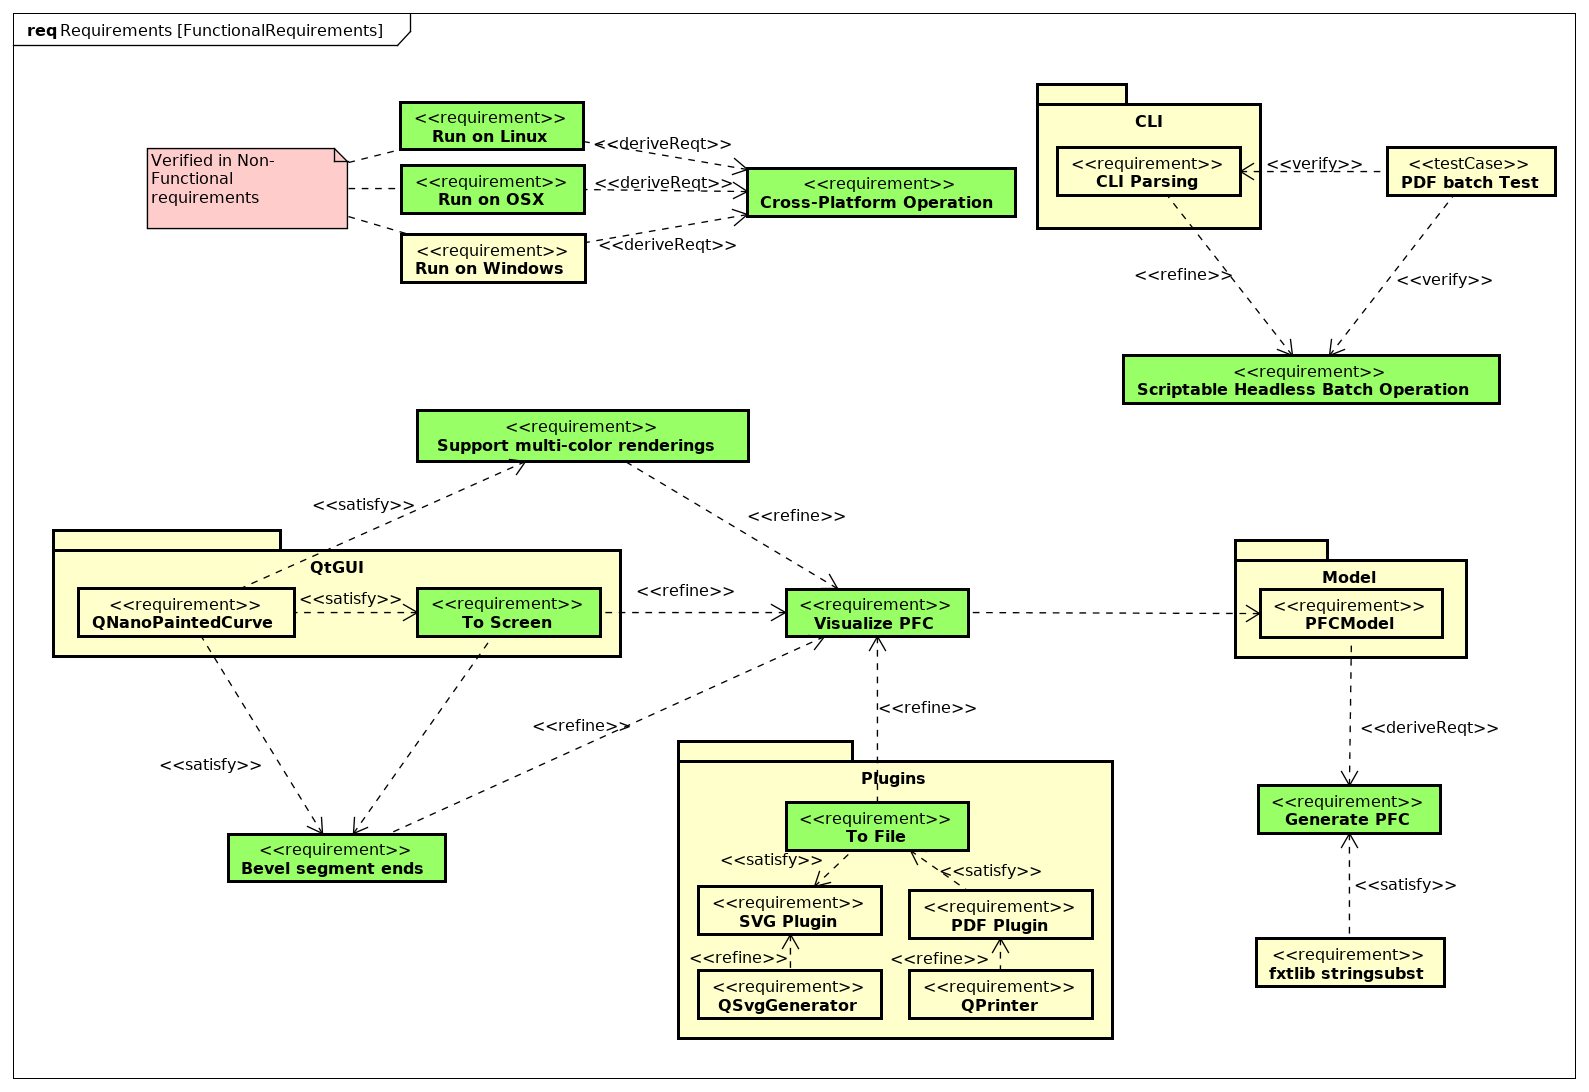
\includegraphics[width=\textwidth]{FunctionalRequirements}
	\caption{Functional requirements}
	\label{fr}
\end{figure}

\begin{figure}[p]
	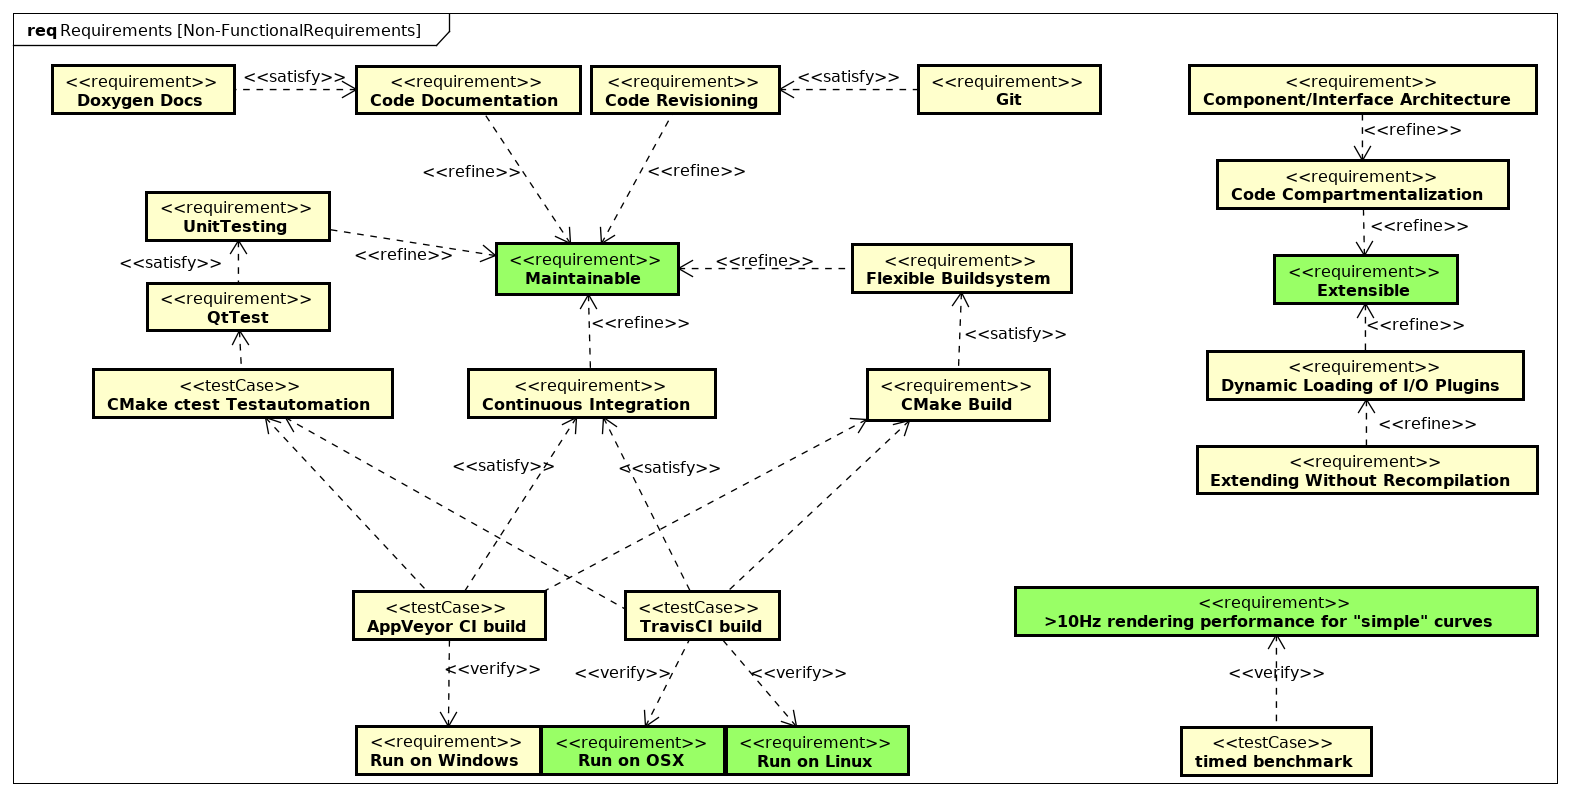
\includegraphics[width=\textwidth]{Non-FunctionalRequirements}
	\caption{Non-functional requirements}
	\label{nfr}
\end{figure}


\subsubsection{Dynamic Library Loading}



To get cross-\gls{os} operation without recompiling, use Qt's Library loading mechanism: QPluginLoader

\subsubsection{Signals and Slots in QML}
Signals are captured by invoking Signal Handlers

\subsubsection{Qt and C++1y}
Move semantics not implemented
QQuickItem has disabled copy ctor and no move ctor
use unique\_ptrs to copy without resource leaks

\section{Flexible Buildsystem}
Due to the requirement of a Multi-platform architecture, one of the first considerations is how to get the program code built.

Though it would surely be possible to have the platform agnosstic sources present, and then manually create a project for MSVC/MinGW when on Windows, gnu gcc on Linux and clang on Mac, this would be a pain to set up and maintain.

Solutions to this problem exist in so-called buildsystem generators. Those gather sources, dependencies and additional project information from a configuration file, detect the architecture they are running on, and generate the files necessary to compile the full project on whichever compiler is present on the current system.

QMake - The native buildsystem generator of Qt, uses .pro files for project description

CMake - A powerful and scalable config script-driven generator that is widely used in both Open Source and commercial projects 


\section{Commandline Parsing}
Unlike other programming languages (e.g. Python), C++ does not provide a standard built-in facility to provide parsing capability for parsing parameters passed to the program as commandline options.

Alternatives:

\begin{itemize}
\item getopt() - Coming from C, this is a legacy method widely used on Linux. Since it is specific to POSIX systems, it cannot be used on Windows 
\item Boost.progam\_options - A C++ native, highly configurable solution shipped with the open source Boost library
\url{http://www.boost.org/doc/libs/1\_58\_0/doc/html/program\_options.html}
\item QtCommandLineParser - A Qt native parsing class. Batch-parses all parameters and returns data structures with positional arguments in correct order, and a (reordered) map of switches with their parameters
http://doc.qt.io/qt-5/qcommandlineparser.html
\item Manual parsing of the argv array. While this is the most flexible solution in customization, it is reinventing the wheel and also very inflexible with respect to extensibility.
\end{itemize}

Due to it supporting our use-case, being easily extensible and not introducing any more dependencies into the project above the already used Qt Framework libraries, the QtCommandLineParser was chosen to provide the main CLI-based interface to the program.


\section{Option Persistency}
Since it is often unneccessary to set any and all config options for the program on the command line each time it is run, keeping config options persistently over program relaunches is useful. The typical implementation of this persistent store again varies by platform, ranging from putting keys into the Windows registry, over property list files on Mac to plain .ini or .cfg files on Linux.

Again, Qt comes with a wrapper around this platform disparity
